\documentclass{article}
\usepackage{tikz}
\usepackage{amsthm}

\theoremstyle{definition}
\newtheorem*{solution}{Solution}
\title{Counting Set A}
\author{}
\date{}

\begin{document}
\maketitle
\noindent Problems should be solved without calculators unless otherwise 
specified. Remember to explain how you solved a problem.
\begin{enumerate}
    \item In how many ways can the letters $A$, $B$, $C$, and $D$ be arranged so 
        that no letter is adjacent to any letter that comes immediately before 
        it or immediately after it alphabetically?
        \begin{solution}
            If $A$ is in the first spot, then $B$ must be in the third or fourth 
            spot. But if $B$ is in the third spot then it must be next to $C$, 
            and if $B$ is in the fourth spot then $C$ and $D$ are next to each 
            other. Therefore $A$ must not be in the first spot. It also can't be 
            in the last spot for the same reason, so it must be in one of the 
            middle spots. If $A$ is in the second spot, then $B$ must be in the 
            fourth spot, so $C$ must be in the first spot and $D$ must be in the 
            third spot. Therefore there is one way to arrange the letters if $A$ 
            is in the second spot, and another way if $A$ is in the third spot, 
            so in total there are $2$ ways to arrange the letters, which are 
            $BDAC$ and $CADB$.
        \end{solution}
    \item If there are $3$ boys and $4$ girls in a group and two are chosen to 
        give a report, what is the probability that one boy and one girl are 
        chosen?
        \begin{solution}
            First, we'll count the total number of ways to chose two people out 
            of seven. There are $7$ ways to choose the first person and $6$ ways 
            to choose the second person, for a total of $42$ ways. There are $3$ 
            ways to choose a boy, $4$ way to choose a girl, and we can either 
            have a boy first and then a girl or a girl first and then a boy, so 
            there are $3 \cdot 4 \cdot 2 = 24$ ways to choose two people such 
            that one of them is a boy and the other is a girl. Therefore the 
            probability is $\frac{24}{42} = \frac{4}{7}$.

            We can solve this problem in a differnet way if we say that the 
            order doesn't matter. There are $7$ ways to choose the first person 
            and $6$ ways to choose the second person, but we are counting each 
            pair twice since they can be in one of two orders, so we divide by 
            two to get $\frac{7 \cdot 6}{2} = 21$ ways of choosing two people 
            out of seven where order doesn't matter. There are $3$ ways to 
            choose a boy and $4$ ways to choose a girl, so there are a total of 
            $12$ ways to choose a boy and a girl. And the probability is 
            $\frac{12}{21} = \frac{4}{7}$.
        \end{solution}
    \item Cedric has four times as many shirts and pants, and he can use them to make
        100 different shirt-and-pants outfits. How many pants does Cedric have?
        \begin{solution}
            If Cedric has $s$ shirts and $p$ pants, then, according to the 
            Fundamental Counting Principle, he can make $sp$ outfits. Since 
            Cederic has four times as many shirts as pants, we have the equation 
            $4p^2 = 100$. Therefore, $p^2 = 25$, and $p = 5$. So, Cedric has $5$ 
            pants.
        \end{solution}
    \item How many rectangles (of any size) are there in this figure?
        \begin{center}
            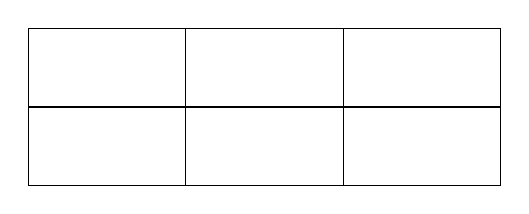
\begin{tikzpicture}
                \draw (0, 0) -- (6, 0) -- (6, 2) -- (0, 2) -- cycle;
                \draw (0, 1) -- (6, 1);
                \draw (2, 0) -- (2, 2);
                \draw (4, 0) -- (4, 2);
            \end{tikzpicture}
        \end{center}
        \begin{solution}
            One way to count the rectangles systematically would be to separate 
            them by size. First, we can count the number of rectangles of size 
            $1$, which is six. Then we count the number of rectangles of size 
            $2$. There are four horizontal ones and three vertical ones. Now we 
            count the rectangles of size $3$. These must be horizontal, and 
            there are two of them. There are two rectangles of size $4$, and one 
            rectangle of size $6$. So in total, there are $18$ rectangles.

            Another way to do this would be to recognize that a rectangle can be 
            defined by the position of its four sides. There are three ways to 
            choose two of the three horizontal lines to be the top and bottom of 
            the rectangle, and there are six ways to choose two of the four 
            vertical lines to be the sides of the rectangle, so there are $3 
            \cdot 6 = 18$ rectangles.
        \end{solution}
    \item Every student who applied for admission to a veterinary school has at 
        least one pet: $30$ have a cat, $28$ have a dog, and $26$ have fish. If 
        $13$ students have a fish and a cat, $15$ students have fish and a dog, 
        $11$ students have both a cat and a dog, and $4$ students have a cat, a 
        dog, and a fish, how many students applied to veterinary school? Hint 1: 
        Use this Venn diagram. Hint 2: The inclusion-exclusion principle can be 
        used for more than two sets. If we added the number of people who have a 
        cat, the number of people who have a fish, and the number of people who 
        have a dog together, how many times is each region in the Venn diagram 
        counted? What can we subtract in order to correct for regions being 
        counted multiple times? What might we need to add back in order to 
        ensure all regions are counted? Try looking up the inclusion-exclusion 
        principle for more hints.
        \begin{center}
            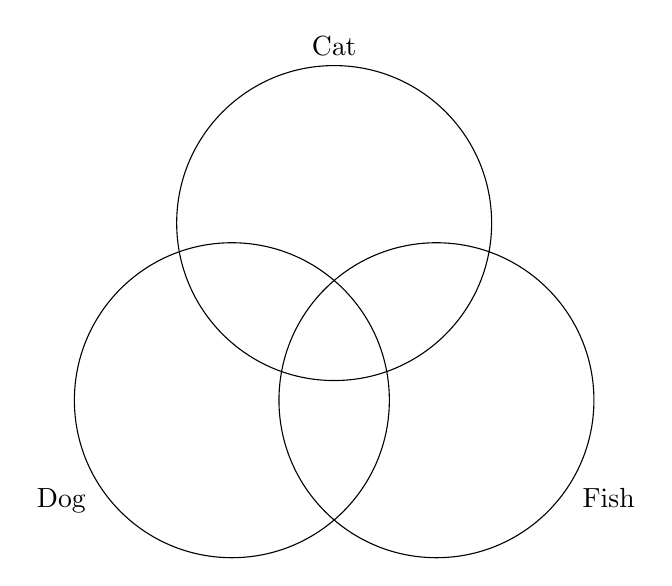
\begin{tikzpicture}
                \draw (90 : 1.5) circle (2);
                \node[above] at (90 : 3.5) {Cat};
                \draw (210 : 1.5) circle (2);
                \node[below left] at (210 : 3.5) {Dog};
                \draw (330 : 1.5) circle (2);
                \node[below right] at (330 : 3.5) {Fish};
            \end{tikzpicture}
        \end{center}
        \begin{solution}
            If we added the areas of the three circles together, we would get 
            $30 + 28 + 26 = 84$, which counts the areas that are in two circles 
            twice, and the area in all three circles three times. To correct 
            this, we can subtract the areas that are in two circles to get $84 - 
            13 - 15 - 11 = 45$. We've added the area in the center three times 
            and subtracted it three times, so it didn't get counted. Therefore 
            we add it back to get $45 + 4 = 48$.
        \end{solution}
\end{enumerate}
\end{document}
